\part*{Trabajo a realizar}\addcontentsline{toc}{part}{Trabajo a realizar}
\section{Trabajo realizado por WildSense y motivación de mejoras}
Para entender la motivación detrás de este proyecto es importante conocer el proceso de estimación de biomasa implementado en WildSense, así como identificar debilidades y posibles soluciones. A continuación se explica el proceso, el cual además es ilustrado en la figura \ref{fig:workflow_wildsense}.

\begin{enumerate}
    \item \textbf{Captura en video}: se registran videos de salmones mediante cámaras estéreo, obteniendo información visual, mapas de profundidad y nubes de puntos.
    \item \textbf{Detección y segmentación}: las imágenes se someten a un procesamiento mediante modelos de segmentación de instancias, que generan predicciones referentes a la posición (detección) y al contorno (segmentación) de los peces presentes en la escena. Este procedimiento posibilita el aislamiento de información visual y espacial correspondiente a los objetos de interés ---salmones en este caso--- del fondo.
    \item \textbf{Tracking}: con el fin de mitigar errores derivados de mediciones únicas, se implementa una estimación estadística basada en múltiples muestras, lo que requiere agrupar las predicciones correspondientes a cada pez. La agrupación se logra mediante algoritmos de seguimiento o ``tracking''. Si bien en ocasiones la tarea de seguimiento se integra al proceso de detección en videos, en el caso de WildSense, se utilizan modelos YOLO que procesan imágenes de forma independiente sin incluir seguimiento. Por el elevado costo computacional que implicaría incorporar un modelo adicional específico para el seguimiento, se opta por utilizar la técnica de seguimiento basado en detección, aprovechando las detecciones ya obtenidas.
    \item \textbf{Post-procesado}: se realiza filtrado de muestras deficientes. Estas constituyen casos donde el pez está incompleto, cubierto, muy alejado para realizar una estimación apropiada o el número de muestras rastreadas son muy pocas.
    \item \textbf{Estimación de volumen}: finalmente se toman los datos de profundidad tomados con las cámaras estéreo y se emparejan a modelos tridimensionales creados en Blender, con los cuales es posible realizar estimaciones de volumen y masa.
\end{enumerate}

\begin{figure}[tb]
\begin{center}
    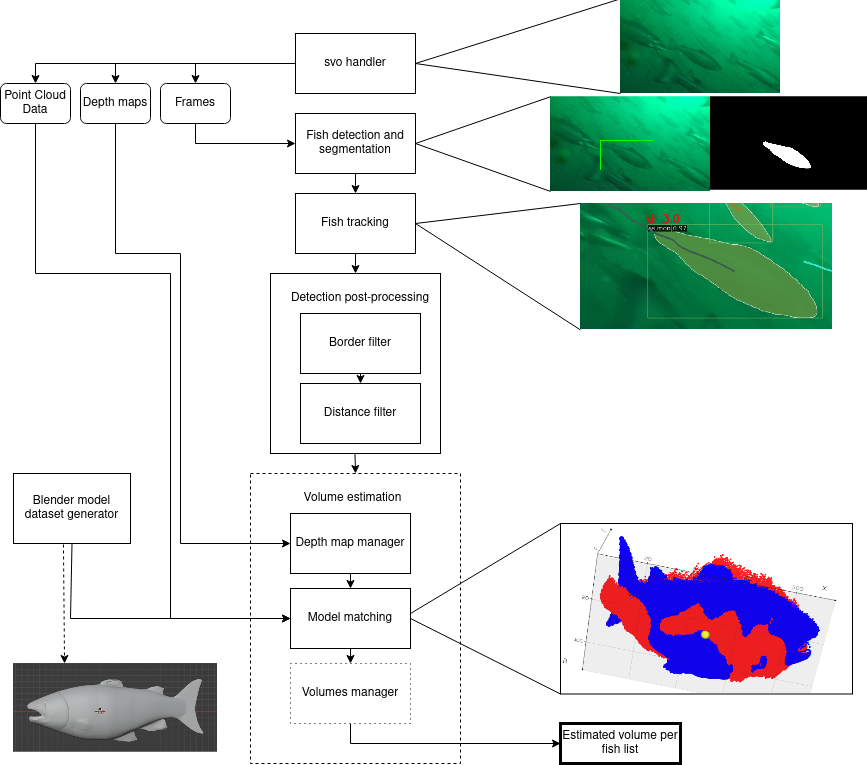
\includegraphics[width=0.8\textwidth]{figures/workflow_wildsense.png}
    \caption[Flujo de trabajo implementado por WildSense para estimación de masa y volumen en peces]{Diagrama de flujo con el proceso estimación de volumen y biomasa de salmones implementada por WildSense \cite{wildsense-2}.}
    \label{fig:workflow_wildsense}
\end{center}
\end{figure}

Cabe mencionar que las etapas de seguimiento y filtrado de detecciones resultan computacionalmente costosas y dado que muchas predicciones son eventualmente descartadas, sería preferible excluirlas desde un principio evitando segmentarlas del todo. Otro problema que existe es el “parpadeo”, que consiste en instancias segmentadas de forma intermitente a lo largo de un video, resultando en seguimientos truncados, lo que hace que sean excluidos de las estimaciones o, en caso de no serlo, reducen la información disponible por estimación, deteriorando su calidad.

Estos problemas justifican la creación de una base de datos que contenga únicamente instancias de interés, con el fin de disminuir el costo computacional en la etapa de post-procesado. Se espera además, que los modelos entrenados se especialicen en segmentar exclusivamente los peces de interés, reduciendo la omisión de instancias relevantes, en consecuencia, minimizando el “parpadeo”, mejorando la calidad del seguimiento y en consecuencia de las estimaciones.